\section{Methodology}
\label{sec:method}


\subsection{Velocity (Digital)}

\begin{figure}[H]
	\centering
	\makebox[\linewidth][c]{
	\begin{tikzpicture}
		\node[inner sep=0pt] (img) at (0,0) {	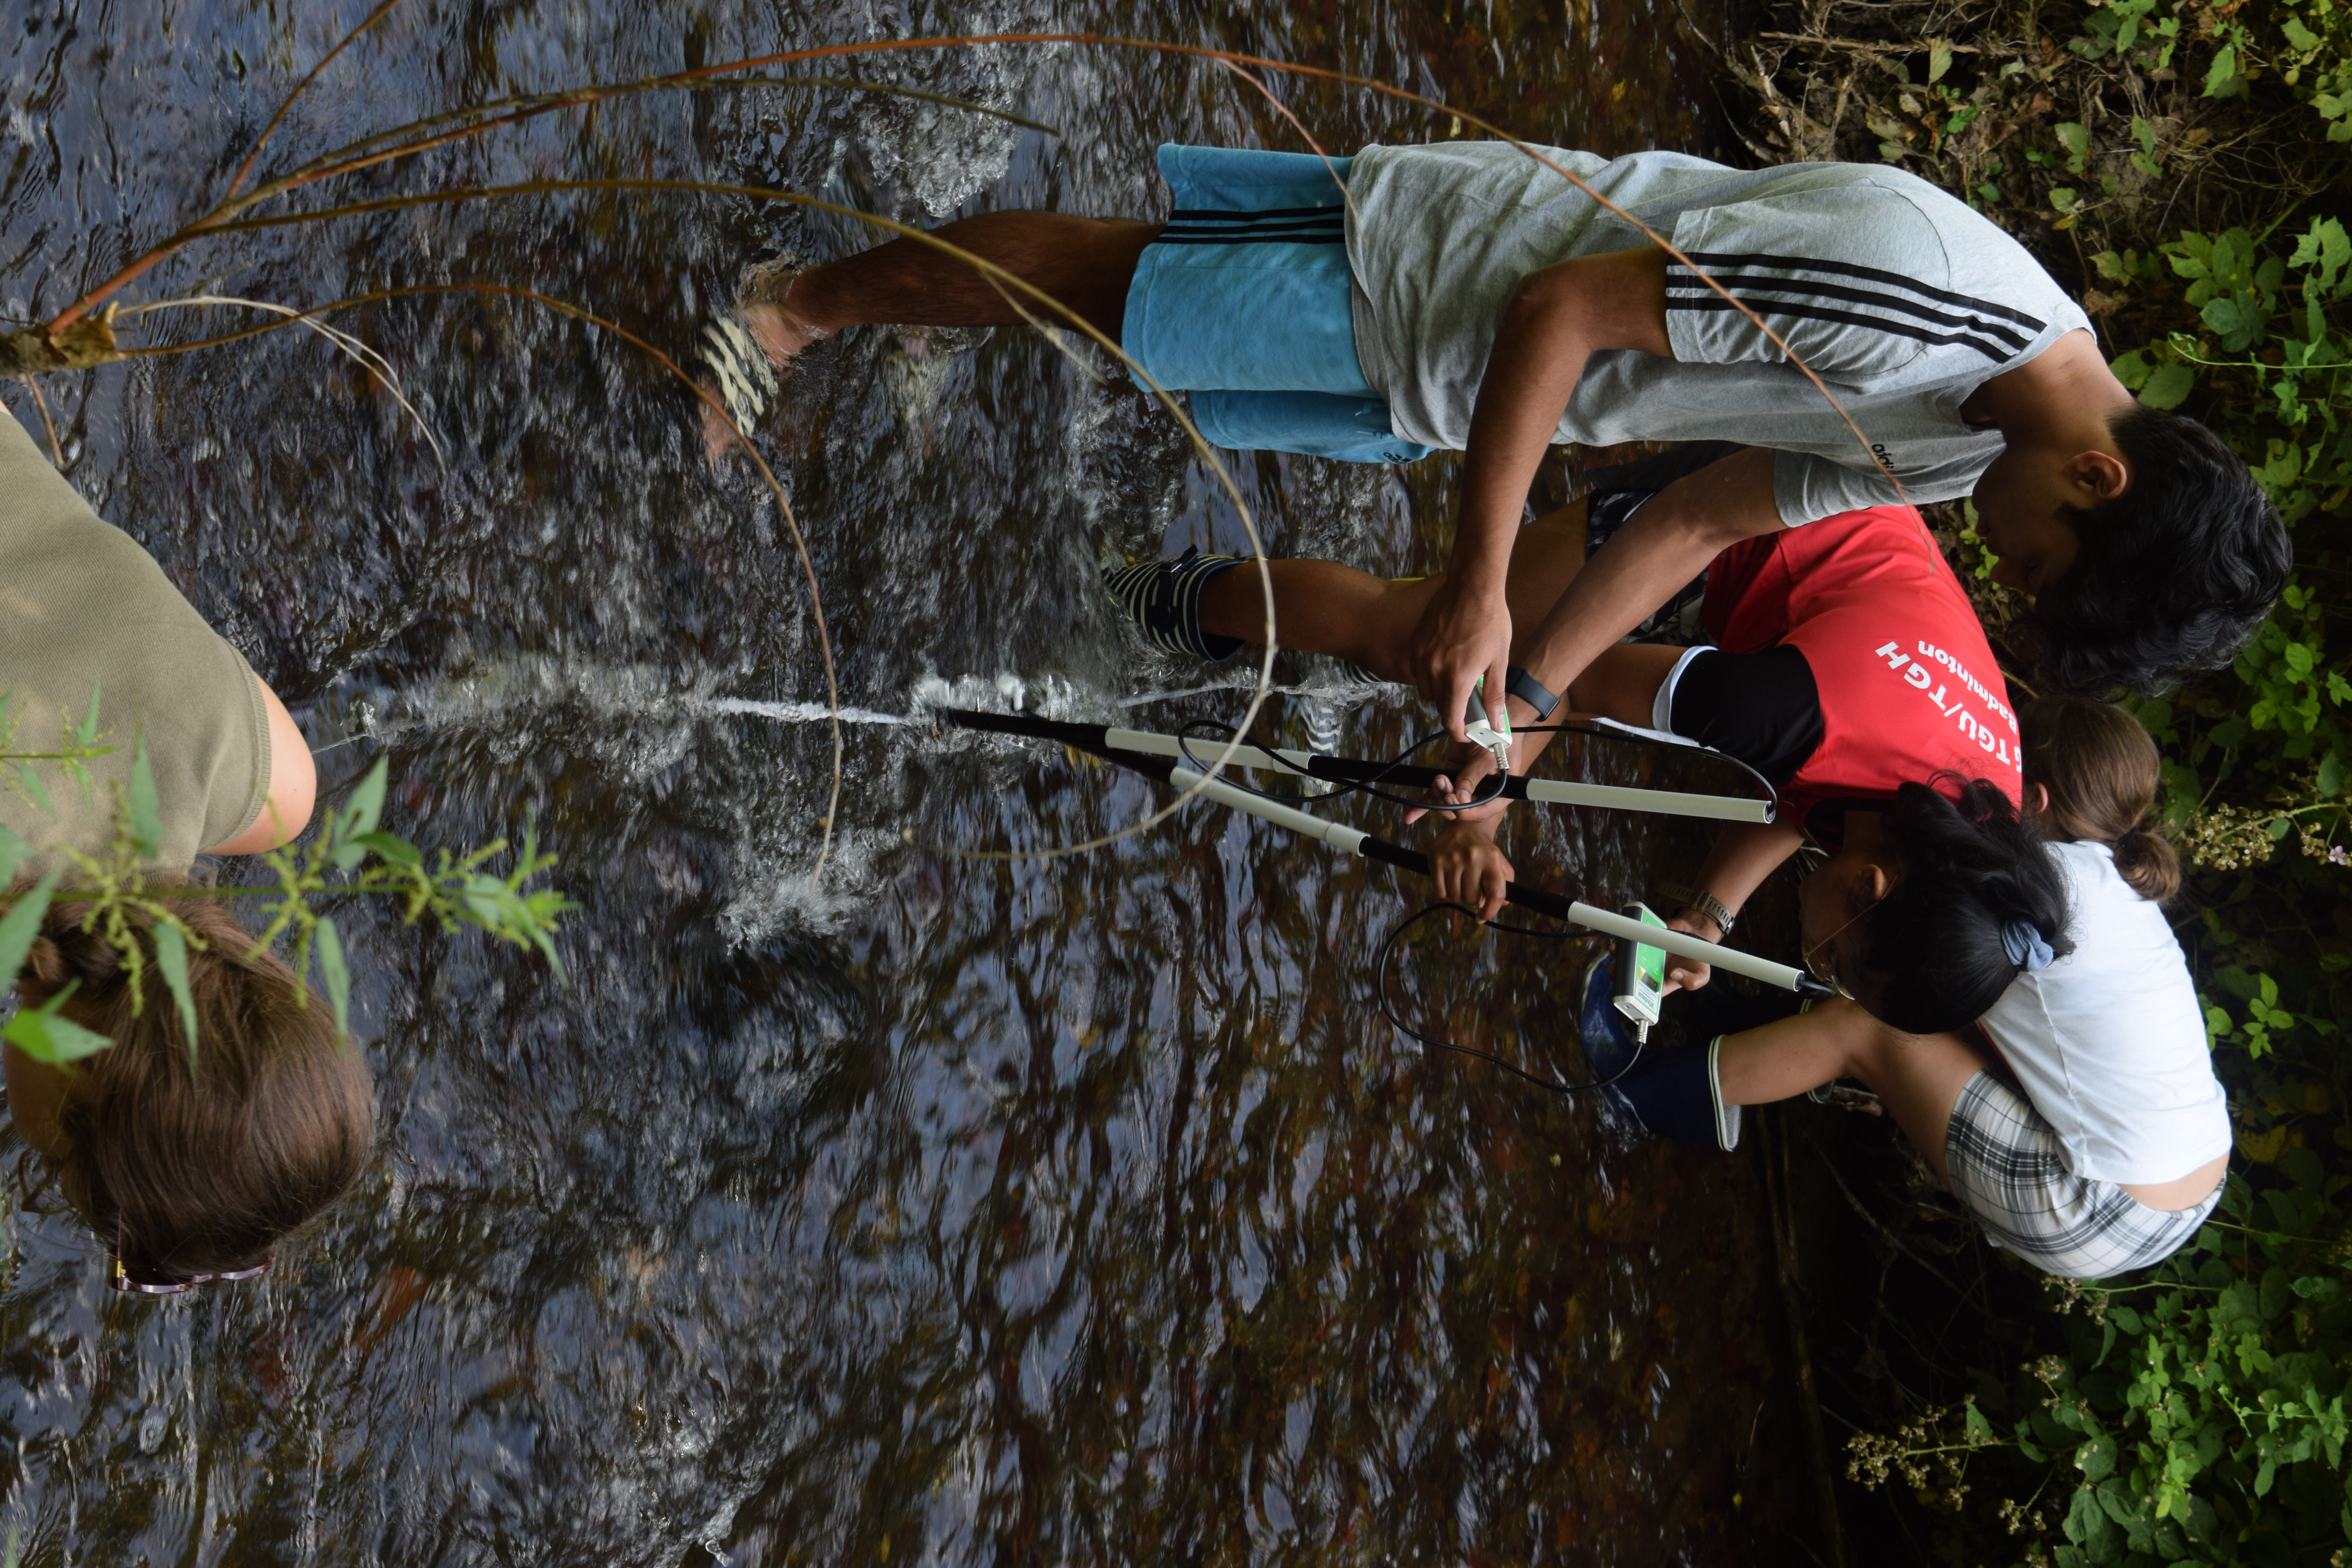
\includegraphics[width=0.7\textwidth, angle=90]{Images/digitalvelo_3.jpg}};
		
		%right
		\draw[->, line width=2pt, color=red] (6.9, 0) -- (-0.35, -0.64);
		\node[draw, fill=white, line width=1pt, anchor=west, align=left] at (7, 0) {Digital Flowmeter};
		
		\draw[->, line width=2pt, color=red] (5.6, 4) -- (0.45, 3.0);
		\node[draw, fill=white, line width=1pt, anchor=west, align=left] at (5.7, 4) {Measured at River \\ Bank along water surface};
		
		%left
		\draw[->, line width=2pt, color=red] (-4.9, 3) -- (-0.28, -1.8);
		\node[draw, fill=white, line width=1pt, anchor=east, align=left] at (-5, 3) {Measuring Tape};
		
			%left
		\draw[->, line width=2pt, color=red] (-4.7, 1) -- (-0.4, -2.5);
		\node[draw, fill=white, line width=1pt, anchor=east, align=left] at (-4.8, 1) {Tape meaure not taut \\ due to high velocity of river \\ exerting force};
		
	\end{tikzpicture}}
	\caption{Digital Velocity measured at Site 3.}
\end{figure}

Velocity was measured in two ways for the following investigation, digital and analogue. To measure digitally, first the width of the river channel was measured at each site and the middle of the channel was recorded. This middle point in the river was where the flow-meter was placed at the surface, with the propeller facing against the flow, in order to measure the velocity as a form of \textbf{purposive sampling}\footnote{\textbf{Purposive sampling} is when a sample is chosen based on a predetermined feature, which is beneficial to the outcome of the study.}.

\clearpage

\[
\textbf{Velocity Equation when digital flow-meter is not used:} 
\]
\[
v = \frac{\Delta s}{\Delta t}
\qquad\qquad
\begin{aligned}
	v &= \text{velocity (m/s)} \\
	\Delta s &= \text{change in distance (m)} \\
	\Delta t &= \text{change in time (s)}
\end{aligned}
\]


Purposive sampling is used, as the least drag is present in the middle of the river channel and away from the river bed, which is a pre-defined characteristic chosen for higher accuracy. This was measured 4 times as the data kept fluctuating by one decimal point, then the average was calculated. A digital flow-meter was used for the data as it is more accurate than an analogue measurements as obstacles in the river, can halt or alter the flow of the float. 

\subsection{Channel Width}

\begin{figure}[H]
	\centering
	\includegraphics[width=1.0\textwidth]{Images/WidthAcc.jpg}
	\caption{Measurement of Channel width in middle course.}
\end{figure}

Measurement of the channel width was taken by using a tape measure. The tape measure was placed perpendicular to river flow and the measurement was taken from river bank to river bank at the points where the water meets the bank. During this the tape measure was pulled taut across the water surface before the measurements were taken. There were 3 measurements made for width and the sampling technique used was pragmatic sampling.

This method of sampling was used as the point in the sites chosen to measure width were chosen as they were the most accessible with the least amount of obstructions, which would cause uncertainties.


\subsection{Channel Depth}

\begin{figure}[H]
	\centering
	\includegraphics[width=0.75\textwidth]{Images/DepthAcc.jpg}
	\caption{Depth measurements taken at river}
	\label{fig:Depth}
\end{figure}

Measurement of the channel depth was taken through the use of a meter rule. A tape measure spanning the width of the river was placed in order to provide the overall width, which would then help determine the intervals at which to measure the depth across the river channel. The meter rule was placed with its narrower side exposed to river flow and the distance between the water surface and the riverbed was measured and recorded. 

Pragmatic sampling was also utilised here as places that had fewer significant protrusions in the river bed, such as large rocks, were avoided to allow for a more accurate measurement of the river bed. These measurements were taken 3 times at each interval and had the average calculated for each of the intervals. Then for the overall depth, the mean of the averages was used.

\subsection{Cross-Sectional Area}

Cross-sectional area is measured by multiplying the mean width with the mean depth.

	\begin{align*}
	A &= \text{Mean Width} \times \text{Mean Depth} \\
	A_{\text{Site 1}} &= 2.02 \times 0.145 = 0.2929 \text{ m$^2$} \\
	\end{align*}
	


\subsection{Channel Efficiency}


\begin{enumerate}
	\item Channel efficiency = Hydraulic radius -> The higher the radius, the greater the efficiency.
	\item $\text{Cross-Sectional Area}\div\text{Wetted Perimeter} = \text{Hydraulic Radius}$
\end{enumerate}


\begin{align*}
	R &= \frac{A}{P} \\
	R_{\text{Site 1}} &= \frac{0.2929}{2.03} = \text{0.144 m (3 s.f.)} \\
\end{align*}

\subsection{River Discharge}

$\text{Discharge (cumecs)}= \text{Cross-Sectional Area}\ (\si{\metre\squared}) \times \text{Velocity}\ (\si{\metre\per\second})$

The mean depth and mean width are first used to measure cross-sectional area (\si{\metre\squared}), then the velocity is measured through either a digital flow-meter or with a stopwatch, a cork,measuring tape and ranging poles ($\times 4$). Then the average velocity is taken and multiplied by the area to get the discharge fo the river.


\begin{align*}
	Q &= A \times \text{v} \\
	Q_{\text{Site 1}} &= 0.2929 \times 0.5725 = 0.168 (3 s.f.) \text{ m$^3$/s} \\
\end{align*}

\subsection{Bedload Size}

\begin{figure}[H]
	\centering
	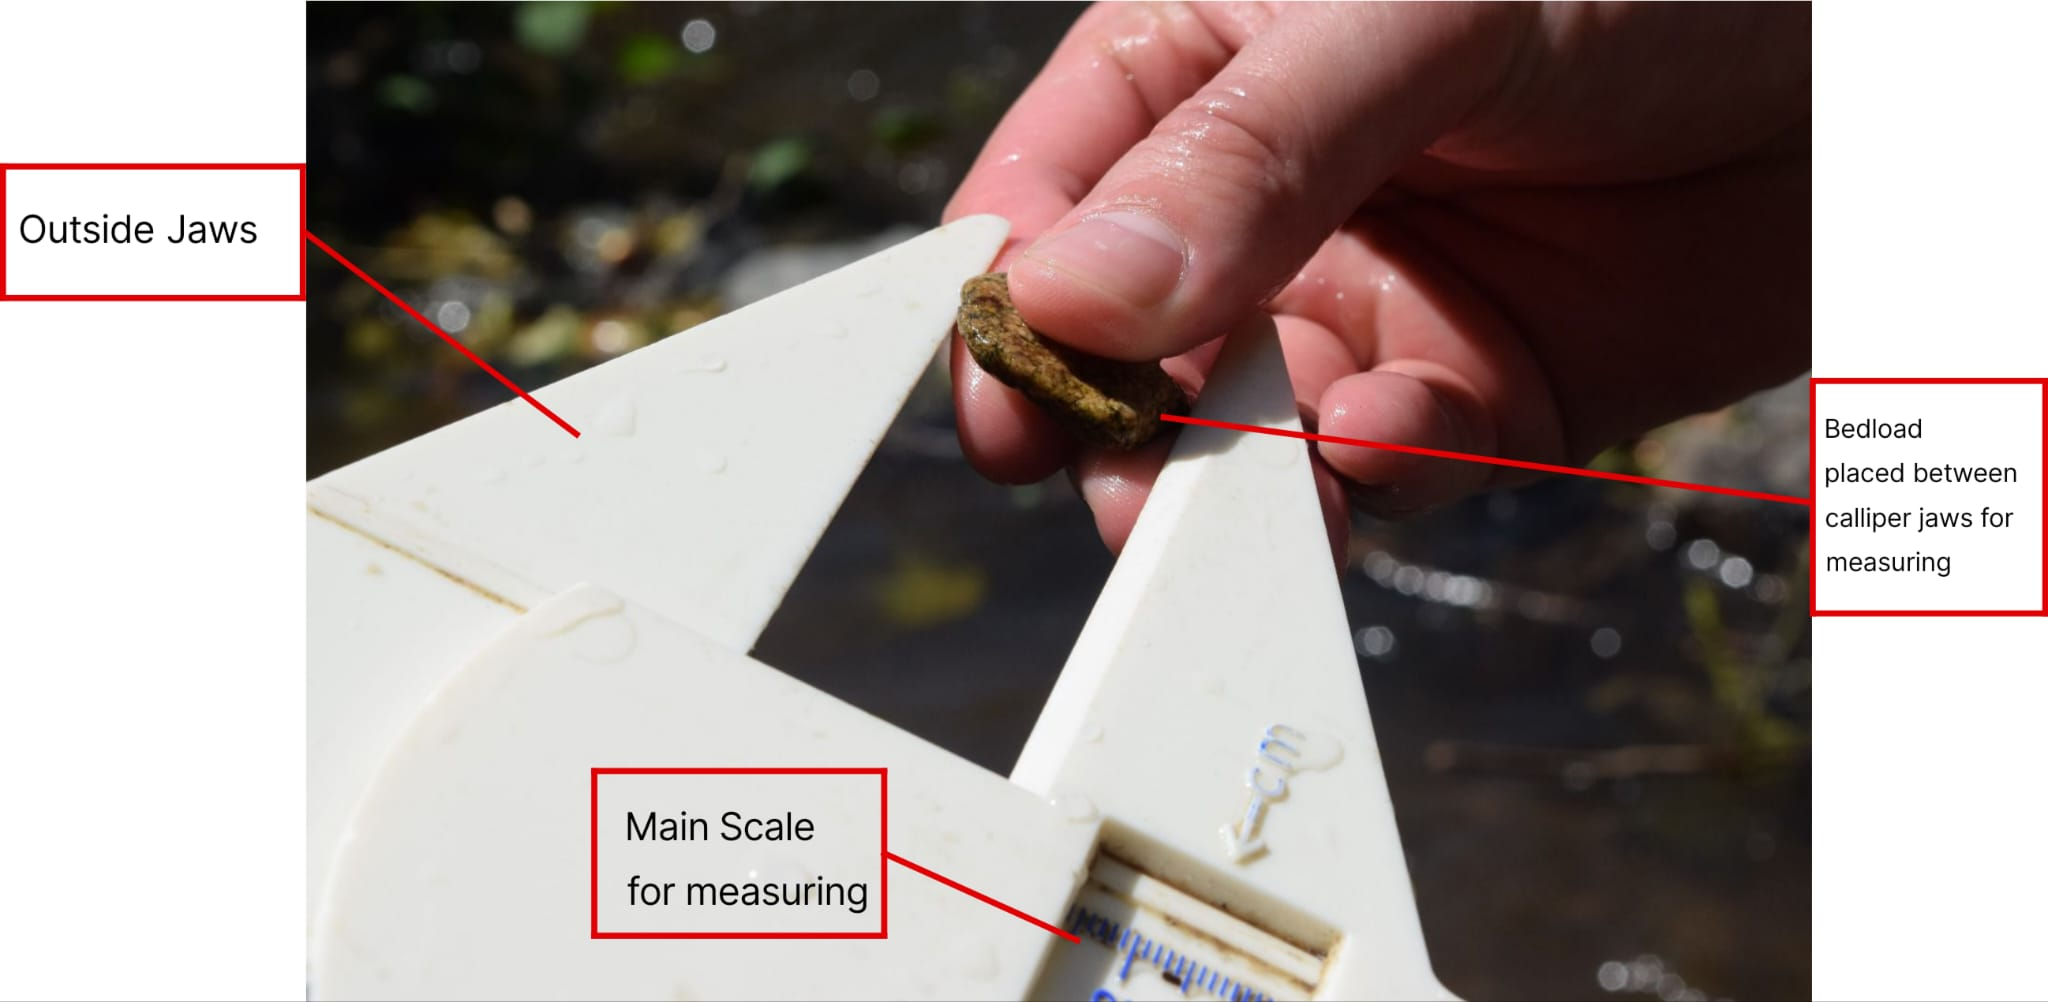
\includegraphics[width=0.9\textwidth]{Images/Bedloadmeasacc.jpg}
\end{figure}

To measure bedload size, a calliper was used and measurements on the chosen rock's length, width and breadth were taken. These results were then averaged and recorded on a table. 10 samples were measure at every site, the averages of the average sizes of these samples were taken in order to determine the average bedload size at each site.

Systematic sampling was used in this case so as to broaden the variety of bedload samples used to be measured in order to provide a higher level of accuracy.



